\documentclass{standalone}
\usepackage{tikz}

\begin{document}

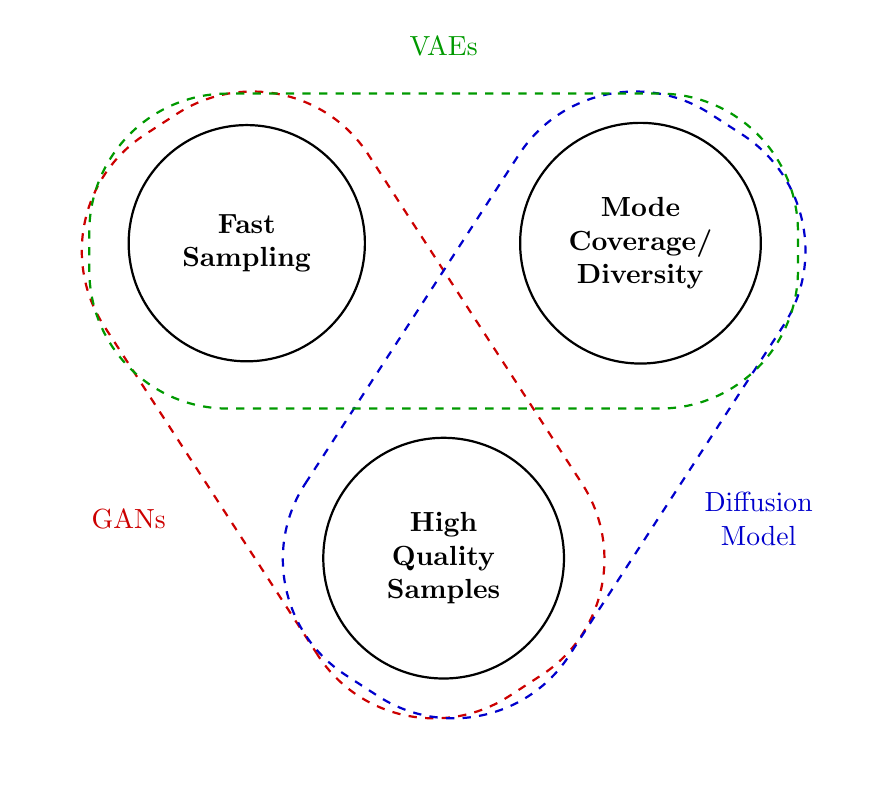
\begin{tikzpicture}
    % Define colors
    \colorlet{myred}{red!80!black}
    \colorlet{myblue}{blue!80!black}
    \colorlet{mybluee}{myblue!80!black}
    \colorlet{mygreen}{green!60!black}
    \colorlet{myorange}{orange!70!red!60!black}
    \colorlet{mydarkred}{red!20!black}
    \colorlet{mydarkblue}{blue!40!black}
    \colorlet{mydarkgreen}{green!20!black}
    
    % Define circle positions
    \coordinate (A) at (-2.5,2);  % Top left
    \coordinate (B) at (2.5,2);   % Top right
    \coordinate (C) at (0,-2);   % Bottom
    
    % Draw the three main circles
    \foreach \pos/\label in {(A)/{\textbf{Fast}\\\textbf{Sampling}},(B)/{\textbf{Mode}\\\textbf{Coverage/}\\\textbf{Diversity}},(C)/{\textbf{High}\\\textbf{Quality}\\\textbf{Samples}}} {
        \node[circle, draw=black, fill=white, thick, minimum size=3cm, text width=2.5cm, align=center] at \pos {\label};
    }
    
    % Draw the dashed ellipses
    % Red (left) ellipse
    \draw[myred, dashed, rounded corners=50pt, rotate=33, xshift = 1.4cm, yshift=-0.6cm, thick] (-4.5,-3) rectangle (-0.5,5.5);

    % Red (left) ellipse
    \draw[myblue, dashed, rounded corners=50pt, rotate=-33, xshift = 3.6cm, yshift=-0.6cm, thick] (-4.5,-3) rectangle (-0.5,5.5);
    
    \draw[mygreen, dashed, rounded corners=50pt, rotate=90, xshift = 4.4cm, yshift=-1.5cm, thick] (-4.5,-3) rectangle (-0.5,6);
    
    % Add placeholder text
    \node[myred] at (-4,-1.5) {GANs};
    \node[myblue, align=center] at (4,-1.5) {Diffusion \\ Model};
    \node[mygreen] at (0,4.5) {VAEs};
    
\end{tikzpicture}

\end{document}


    
    
    